% =====================================================================
%  Linen Connections - Inbox + Automation Pitch
%  Compile with: pdflatex (works on Overleaf)
%  This deck is designed to be simple, visual, and client-friendly.
% =====================================================================
\documentclass[aspectratio=169,11pt]{beamer}

\usepackage[utf8]{inputenc}
\usepackage{tikz}
\usepackage{pgfplots}
\usepackage{amssymb}
\usepackage{textcomp}
\pgfplotsset{compat=1.18}
\usetikzlibrary{arrows.meta,positioning,shapes.geometric,calc}

% ---------- Colour palette -------------------------------------------
\definecolor{ink}{HTML}{2B2B2B}
\definecolor{teal}{HTML}{1F6F6B}
\definecolor{terra}{HTML}{C8744B}
\definecolor{sand}{HTML}{F3EDE3}
\definecolor{cream}{HTML}{FBF7EF}
\definecolor{muted}{HTML}{7C7C7C}
\definecolor{softgreen}{HTML}{DCEBE7}
\definecolor{softterra}{HTML}{F0D9CB}
\definecolor{gold}{HTML}{D9A441}
\definecolor{danger}{HTML}{B94B4B}

% ---------- Theme -----------------------------------------------------
\usetheme{default}
\usecolortheme{default}
\setbeamertemplate{navigation symbols}{}
\setbeamercolor{background canvas}{bg=cream}
\setbeamercolor{normal text}{fg=ink}
\setbeamercolor{structure}{fg=teal}
\setbeamercolor{title}{fg=teal}
\setbeamercolor{frametitle}{fg=teal}
\setbeamercolor{itemize item}{fg=terra}
\setbeamercolor{itemize subitem}{fg=terra}
\setbeamercolor{block title}{fg=white,bg=teal}
\setbeamercolor{block body}{bg=sand}
\setbeamerfont{frametitle}{series=\bfseries,size=\Large}
\setbeamerfont{title}{series=\bfseries}
\setbeamertemplate{itemize item}{\textbullet}

% ---------- Frametitle + footer --------------------------------------
\setbeamertemplate{frametitle}{%
  \vspace*{0.45em}%
  \hbox{\hspace*{0.35em}\usebeamerfont{frametitle}\usebeamercolor[fg]{frametitle}\insertframetitle}%
  \vspace*{0.15em}%
  \hbox{\hspace*{0.35em}\textcolor{terra}{\rule{2.4em}{2.2pt}}}%
  \vspace*{0.15em}%
}

\setbeamertemplate{footline}{%
  \hfill\textcolor{muted}{\scriptsize\insertframenumber\,/\,\inserttotalframenumber}\hspace*{1em}\vspace*{0.55em}%
}

% ---------- Reusable styles ------------------------------------------
\tikzset{
  card/.style={rectangle,rounded corners=5pt,draw=teal,thick,fill=sand,align=center,inner sep=7pt},
  cardwhite/.style={rectangle,rounded corners=5pt,draw=teal!55,thick,fill=white,align=center,inner sep=7pt},
  route/.style={rectangle,rounded corners=5pt,draw=teal,thick,fill=softgreen,align=center,minimum height=0.95cm,minimum width=2.55cm,font=\small\bfseries},
  arrow/.style={-{Stealth[length=2.5mm]},thick,teal},
  smallnote/.style={font=\scriptsize,text=muted,align=center}
}

% ---------- Picture macros -------------------------------------------
\newcommand{\MailPic}[2]{%
\begin{tikzpicture}[scale=#1]
  \draw[fill=#2,draw=teal,thick,rounded corners=3pt] (0,0) rectangle (2.4,1.45);
  \draw[teal,thick] (0.08,1.32) -- (1.2,0.58) -- (2.32,1.32);
  \draw[teal,thick] (0.08,0.12) -- (0.92,0.78);
  \draw[teal,thick] (2.32,0.12) -- (1.48,0.78);
\end{tikzpicture}%
}

\newcommand{\RobotPic}{%

\begin{tikzpicture}[scale=0.85]
  \draw[teal,thick] (0,0) circle (0.08);
  \draw[teal,thick] (0,-0.08) -- (0,-0.35);
  \draw[fill=softgreen,draw=teal,thick,rounded corners=4pt] (-0.75,-1.25) rectangle (0.75,-0.35);
  \fill[teal] (-0.35,-0.72) circle (0.07);
  \fill[teal] (0.35,-0.72) circle (0.07);
  \draw[teal,thick] (-0.3,-1.02) -- (0.3,-1.02);
\end{tikzpicture}%
}

\newcommand{\PersonPic}{%

\begin{tikzpicture}[scale=0.9]
  \draw[fill=softterra,draw=terra,thick] (0,0) circle (0.34);
  \draw[fill=softterra,draw=terra,thick,rounded corners=7pt] (-0.55,-1.25) rectangle (0.55,-0.38);
\end{tikzpicture}%
}

\newcommand{\Sticker}[2]{%
\begin{tikzpicture}[baseline=-0.6ex]
  \node[rectangle,rounded corners=2pt,fill=#1,draw=#1!70!black,text=white,font=\scriptsize\bfseries,inner xsep=5pt,inner ysep=2pt] {#2};
\end{tikzpicture}%
}

% ---------- Title metadata -------------------------------------------
\title{From Inbox Noise to Business Automation}
\subtitle{A simple first win, then a safer automation roadmap for Linen Connections}
\author{Prepared by IT \& Automation Support}
\date{}

% =====================================================================
\begin{document}

% ---- 1. Title --------------------------------------------------------
{
\setbeamercolor{background canvas}{bg=sand}
\begin{frame}[plain]
  \vspace{0.8cm}
  \begin{center}
    {\Huge\bfseries\textcolor{teal}{From Inbox Noise}}\\[0.15em]
    {\Huge\bfseries\textcolor{terra}{to Business Automation}}\\[0.55em]
    \textcolor{terra}{\rule{5em}{2.5pt}}\\[0.8em]
    {\large\textcolor{ink}{Clean the inbox first. Then build safer AI around the business.}}\\[1.6em]
    
\begin{tikzpicture}[scale=0.95]
      \node at (0,0) {\MailPic{0.75}{white}};
      \node at (2.2,0) {\RobotPic};
      \draw[arrow] (0.9,0) -- (1.45,0);
      \node at (4.2,0) {\PersonPic};
      \draw[arrow] (2.9,0) -- (3.45,0);
      \node[font=\small\bfseries,text=teal] at (6.4,0) {n8n workflows};
      \draw[arrow] (4.9,0) -- (5.65,0);
    \end{tikzpicture}\\[1.7em]
    {\footnotesize\textcolor{muted}{For orders@linenconnections.com.au and future customer-service operations}}
  \end{center}
\end{frame}
}

% ---- 2. Core message -------------------------------------------------
\begin{frame}{The simple story}
  \vspace{0.25cm}
  \begin{center}
  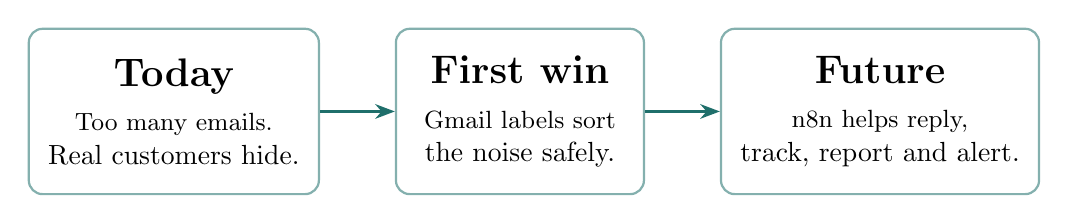
\begin{tikzpicture}[node distance=0.95cm]
    \node[cardwhite,minimum width=3.15cm,minimum height=2.1cm] (now) {\Large\bfseries Today\\[0.4em]\small Too many emails.\\Real customers hide.};
    \node[cardwhite,right=of now,minimum width=3.15cm,minimum height=2.1cm] (first) {\Large\bfseries First win\\[0.4em]\small Gmail labels sort\\the noise safely.};
    \node[cardwhite,right=of first,minimum width=3.15cm,minimum height=2.1cm] (future) {\Large\bfseries Future\\[0.4em]\small n8n helps reply,\\track, report and alert.};
    \draw[arrow] (now) -- (first);
    \draw[arrow] (first) -- (future);
  \end{tikzpicture}
  \end{center}
  \vspace{0.55cm}
  \begin{block}{The pitch in one sentence}
    I can start with a low-risk inbox cleanup, then grow it into a practical automation system that saves time, catches urgent issues, and keeps humans in control.
  \end{block}
\end{frame}

% ---- 3. Problem number ----------------------------------------------
\begin{frame}{What I found in the inbox}
  \vspace{0.3cm}
  \begin{columns}[T,onlytextwidth]
    \column{0.45\textwidth}
      \begin{center}
      {\fontsize{62}{68}\selectfont\bfseries\textcolor{terra}{65--75\%}}\\[0.35em]
      {\large of the inbox is not a real customer}
      \end{center}
    \column{0.52\textwidth}
      
\begin{tikzpicture}[x=0.11\textwidth,y=1cm]
        \draw[fill=teal,draw=none] (0,0) rectangle (7,1.0);
        \draw[fill=gold,draw=none] (7,0) rectangle (7.5,1.0);
        \draw[fill=terra,draw=none] (7.5,0) rectangle (10,1.0);
        \draw[ink,thick] (0,0) rectangle (10,1.0);
        \node[white,font=\bfseries\small] at (3.5,0.5) {system emails};
        \node[white,font=\bfseries\scriptsize,rotate=90] at (7.25,0.5) {ads};
        \node[white,font=\bfseries\small] at (8.75,0.5) {customers};
        \node[align=center,font=\scriptsize,text=teal] at (3.5,-0.55) {Shopify, AusPost, payouts, reviews};
        \node[align=center,font=\scriptsize,text=terra] at (8.75,-0.55) {people needing help};
      \end{tikzpicture}
      \vspace{0.9cm}
      \begin{block}{Why this matters}
        The team is not just busy. The inbox is noisy. Removing the noise makes the real work easier to see.
      \end{block}
  \end{columns}
\end{frame}

% ---- 4. Visual before/after -----------------------------------------
\begin{frame}{Before and after}
  \begin{center}
  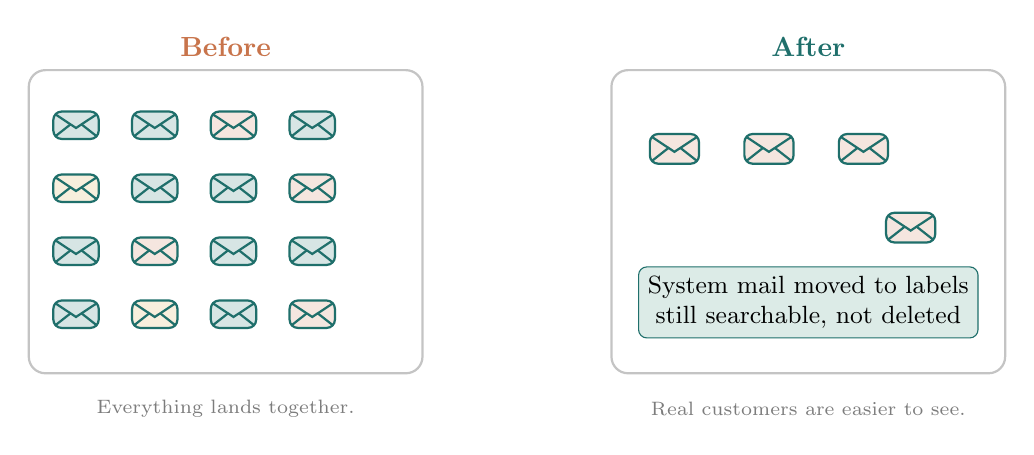
\begin{tikzpicture}
    \node[font=\bfseries,text=terra] at (-3.7,2.35) {Before};
    \node[font=\bfseries,text=teal] at (3.7,2.35) {After};

    \draw[rounded corners=6pt,fill=white,draw=muted!45,thick] (-6.2,-1.8) rectangle (-1.2,2.05);
    \foreach \x/\y/\c in {-5.6/1.35/teal,-4.6/1.35/teal,-3.6/1.35/terra,-2.6/1.35/teal,-5.6/0.55/gold,-4.6/0.55/teal,-3.6/0.55/teal,-2.6/0.55/terra,-5.6/-0.25/teal,-4.6/-0.25/terra,-3.6/-0.25/teal,-2.6/-0.25/teal,-5.6/-1.05/teal,-4.6/-1.05/gold,-3.6/-1.05/teal,-2.6/-1.05/terra} {
      \node at (\x,\y) {\MailPic{0.24}{\c!18}};
    }
    \node[smallnote] at (-3.7,-2.25) {Everything lands together.};

    \draw[rounded corners=6pt,fill=white,draw=muted!45,thick] (1.2,-1.8) rectangle (6.2,2.05);
    \foreach \x/\y in {2.0/1.05,3.2/1.05,4.4/1.05,5.0/0.05} {
      \node at (\x,\y) {\MailPic{0.26}{terra!18}};
    }
    \node[rectangle,rounded corners=3pt,fill=softgreen,draw=teal,align=center,font=\small] at (3.7,-0.9) {System mail moved to labels\\still searchable, not deleted};
    \node[smallnote] at (3.7,-2.25) {Real customers are easier to see.};
  \end{tikzpicture}
  \end{center}
\end{frame}

% ---- 5. What is a label ---------------------------------------------
\begin{frame}{What is a Gmail label?}
  \vspace{0.1cm}
  \begin{columns}[T,onlytextwidth]
    \column{0.42\textwidth}
      \begin{center}
        
\begin{tikzpicture}[scale=1]
          \node at (0,1.35) {\MailPic{0.9}{white}};
          \node[rotate=-8] at (0.9,1.75) {\Sticker{terra}{P1 urgent}};
          \node[rotate=5] at (-0.85,0.9) {\Sticker{teal}{Customer}};
          \node[rotate=-3] at (0.35,0.45) {\Sticker{gold}{AusPost}};
        \end{tikzpicture}
      \end{center}
    \column{0.55\textwidth}
      \begin{block}{Think of a label like a coloured sticker on an email.}
        The email stays in Gmail. The label just tells the team what it is.
      \end{block}
      \vspace{0.25cm}
      \begin{itemize}\setlength\itemsep{0.65em}
        \item It groups similar emails together, like \textbf{Orders}, \textbf{AusPost}, \textbf{Needs Reply}, or \textbf{P1 Urgent}.
        \item It makes work easier to find, search, count and report on.
        \item It can also help Gmail move low-value noise out of the main inbox.
      \end{itemize}
  \end{columns}
\end{frame}

% ---- 6. Gmail filters ------------------------------------------------
\begin{frame}{The first fix: Gmail filters}
  \vspace{0.15cm}
  \begin{center}
  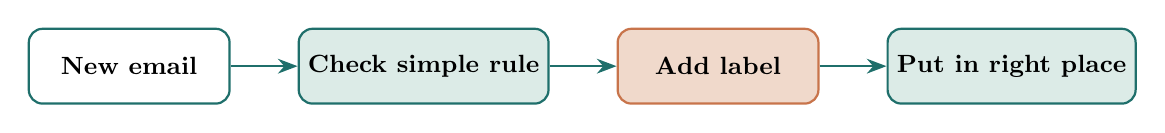
\begin{tikzpicture}[node distance=0.85cm]
    \node[route,fill=white] (email) {New email};
    \node[route,right=of email] (rule) {Check simple rule};
    \node[route,right=of rule,fill=softterra,draw=terra] (label) {Add label};
    \node[route,right=of label] (place) {Put in right place};
    \draw[arrow] (email) -- (rule);
    \draw[arrow] (rule) -- (label);
    \draw[arrow] (label) -- (place);
  \end{tikzpicture}
  \end{center}
  \vspace{0.55cm}
  \begin{columns}[T,onlytextwidth]
    \column{0.47\textwidth}
      \begin{block}{Example rule}
        If sender is Shopify payout email, add \textbf{Shopify Payouts} label and skip inbox.
      \end{block}
    \column{0.47\textwidth}
      \begin{block}{Important safety point}
        Nothing is deleted. Nothing is sent to customers. It only organises the inbox.
      \end{block}
  \end{columns}
\end{frame}

% ---- 7. Safe rollout -------------------------------------------------
\begin{frame}{How we roll it out safely}
  \vspace{0.2cm}
  \begin{center}
  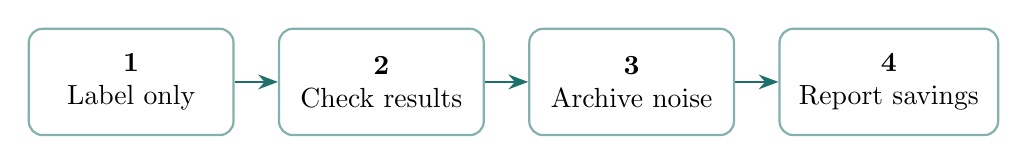
\begin{tikzpicture}[node distance=0.55cm]
    \node[cardwhite,minimum width=2.6cm,minimum height=1.35cm] (a) {\bfseries 1\\Label only};
    \node[cardwhite,right=of a,minimum width=2.6cm,minimum height=1.35cm] (b) {\bfseries 2\\Check results};
    \node[cardwhite,right=of b,minimum width=2.6cm,minimum height=1.35cm] (c) {\bfseries 3\\Archive noise};
    \node[cardwhite,right=of c,minimum width=2.6cm,minimum height=1.35cm] (d) {\bfseries 4\\Report savings};
    \draw[arrow] (a) -- (b);
    \draw[arrow] (b) -- (c);
    \draw[arrow] (c) -- (d);
  \end{tikzpicture}
  \end{center}
  \vspace{0.65cm}
  \begin{itemize}\setlength\itemsep{0.65em}
    \item First, emails get labels but still stay visible.
    \item Then we check that no real customers are trapped in a noise label.
    \item Only after that, safe noise skips the inbox.
    \item The result is measurable: before/after inbox volume and time saved.
  \end{itemize}
\end{frame}

% ---- 8. Why this is convincing --------------------------------------
\begin{frame}{Why this is the right first win}
  \vspace{0.1cm}
  \begin{center}
  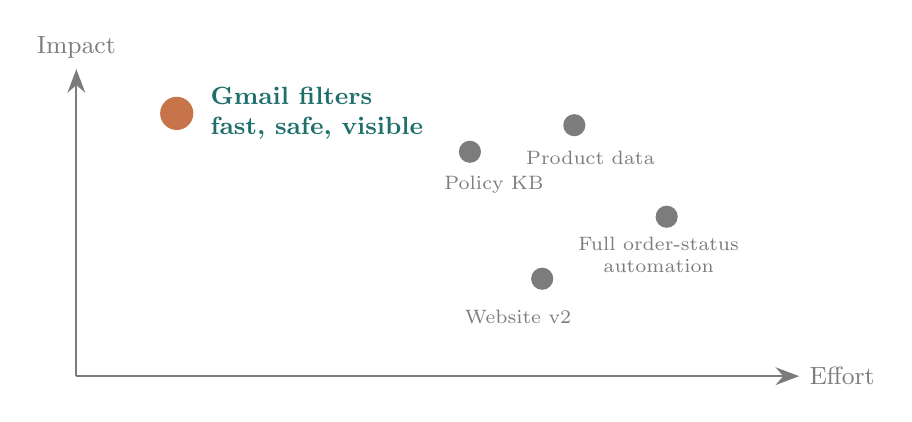
\begin{tikzpicture}[x=1.02cm,y=0.75cm]
    \draw[-{Stealth[length=3mm]},thick,muted] (0,0) -- (9,0) node[right,font=\small]{Effort};
    \draw[-{Stealth[length=3mm]},thick,muted] (0,0) -- (0,5.2) node[above,font=\small]{Impact};
    \fill[terra] (1.25,4.45) circle (6pt);
    \node[anchor=west,align=left,font=\small\bfseries,text=teal] at (1.55,4.45) {Gmail filters\\fast, safe, visible};
    \fill[muted] (4.9,3.8) circle (4pt);
    \node[muted,font=\scriptsize,align=center] at (5.2,3.25) {Policy KB};
    \fill[muted] (6.2,4.25) circle (4pt);
    \node[muted,font=\scriptsize,align=center] at (6.4,3.7) {Product data};
    \fill[muted] (7.35,2.7) circle (4pt);
    \node[muted,font=\scriptsize,align=center] at (7.25,2.05) {Full order-status\\automation};
    \fill[muted] (5.8,1.65) circle (4pt);
    \node[muted,font=\scriptsize,align=center] at (5.5,1.0) {Website v2};
  \end{tikzpicture}
  \end{center}
  \vspace{-0.1cm}
  \begin{block}{It proves value without asking the business to change everything first.}
    Clean inbox first. Then use the cleaner inbox as the base for better automation.
  \end{block}
\end{frame}

% ---- 9. Bigger picture ----------------------------------------------
\begin{frame}{The bigger picture: n8n becomes the engine}
  \vspace{0.1cm}
  \begin{columns}[T,onlytextwidth]
    \column{0.42\textwidth}
      \begin{center}
      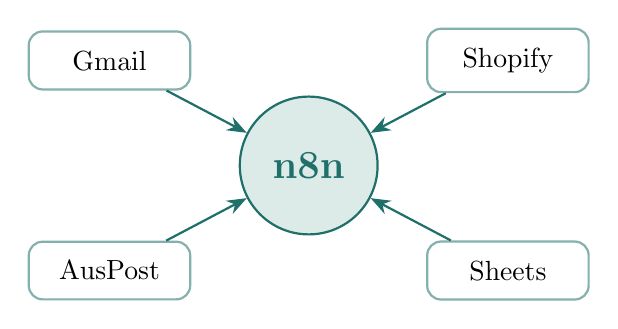
\begin{tikzpicture}[scale=0.92]
        \node[circle,draw=teal,thick,fill=softgreen,minimum size=1.75cm,font=\Large\bfseries,text=teal] (n) at (0,0) {n8n};
        \node[cardwhite,minimum width=2.05cm] (g) at (-2.75,1.45) {Gmail};
        \node[cardwhite,minimum width=2.05cm] (s) at (2.75,1.45) {Shopify};
        \node[cardwhite,minimum width=2.05cm] (a) at (-2.75,-1.45) {AusPost};
        \node[cardwhite,minimum width=2.05cm] (sh) at (2.75,-1.45) {Sheets};
        \draw[arrow] (g) -- (n);
        \draw[arrow] (s) -- (n);
        \draw[arrow] (a) -- (n);
        \draw[arrow] (sh) -- (n);
      \end{tikzpicture}
      \end{center}
    \column{0.55\textwidth}
      \begin{block}{What n8n is, in simple words}
        n8n is a connector. It lets different tools talk to each other and run step-by-step rules automatically.
      \end{block}
      \begin{itemize}\setlength\itemsep{0.6em}
        \item Gmail receives the customer message.
        \item n8n checks facts from trusted systems.
        \item AI can draft or summarise.
        \item A human approves anything risky.
      \end{itemize}
  \end{columns}
\end{frame}

% ---- 10. Current n8n workflow ---------------------------------------
\begin{frame}{Clear picture of the current n8n workflow}
  \vspace{0.05cm}
  \begin{center}
  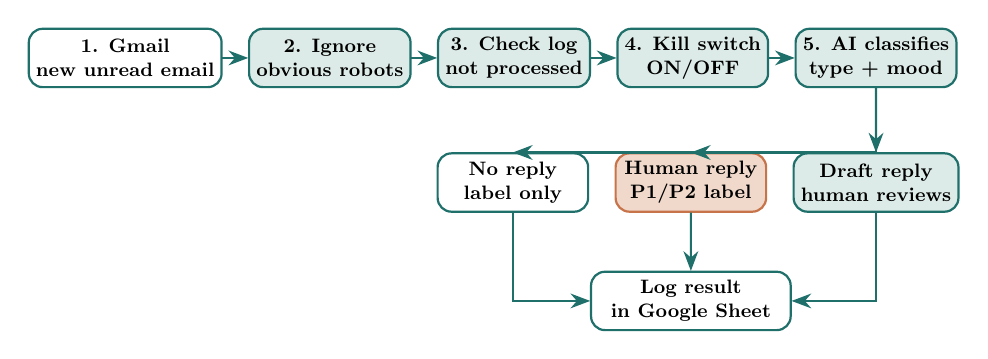
\begin{tikzpicture}[node distance=0.38cm and 0.42cm,scale=0.78,transform shape]
    \node[route,fill=white,minimum width=2.35cm] (inbox) {1. Gmail\\new unread email};
    \node[route,right=of inbox,minimum width=2.35cm] (noise) {2. Ignore\\obvious robots};
    \node[route,right=of noise,minimum width=2.35cm] (dedupe) {3. Check log\\not processed};
    \node[route,right=of dedupe,minimum width=2.35cm] (kill) {4. Kill switch\\ON/OFF};
    \node[route,right=of kill,minimum width=2.35cm] (class) {5. AI classifies\\type + mood};
    \draw[arrow] (inbox) -- (noise);
    \draw[arrow] (noise) -- (dedupe);
    \draw[arrow] (dedupe) -- (kill);
    \draw[arrow] (kill) -- (class);

    \node[route,below=1.05cm of class,fill=softgreen,minimum width=2.45cm] (draft) {Draft reply\\human reviews};
    \node[route,left=of draft,fill=softterra,draw=terra,minimum width=2.45cm] (custom) {Human reply\\P1/P2 label};
    \node[route,left=of custom,fill=white,minimum width=2.45cm] (noreply) {No reply\\label only};
    \node[route,below=0.95cm of custom,fill=white,minimum width=3.25cm] (log) {Log result\\in Google Sheet};
    \draw[arrow] (class) -- (draft);
    \draw[arrow] (class.south) |- (custom.north);
    \draw[arrow] (class.south) |- (noreply.north);
    \draw[arrow] (draft.south) |- (log.east);
    \draw[arrow] (custom) -- (log);
    \draw[arrow] (noreply.south) |- (log.west);
  \end{tikzpicture}
  \end{center}
  \vspace{0.15cm}
  \begin{block}{Safety promise}
    The workflow creates drafts and labels. It does not auto-send customer replies.
  \end{block}
\end{frame}

% ---- 11. Three routes ------------------------------------------------
\begin{frame}{Every email goes into one of three buckets}
  \vspace{0.1cm}
  \begin{center}
  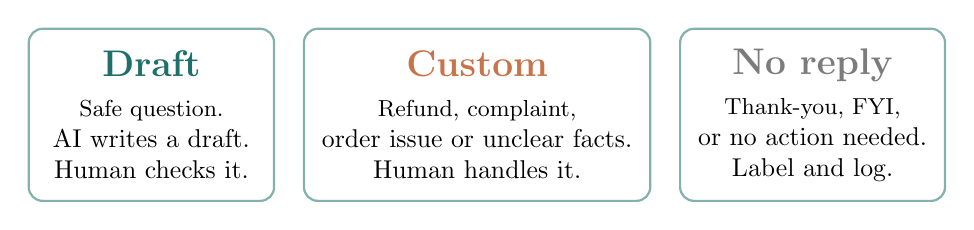
\begin{tikzpicture}[node distance=0.38cm,scale=0.93,transform shape]
    \node[cardwhite,minimum width=3.35cm,minimum height=2.35cm] (draft) {\Large\bfseries\textcolor{teal}{Draft}\\[0.35em]\small Safe question.\\AI writes a draft.\\Human checks it.};
    \node[cardwhite,right=of draft,minimum width=3.35cm,minimum height=2.35cm] (custom) {\Large\bfseries\textcolor{terra}{Custom}\\[0.35em]\small Refund, complaint,\\order issue or unclear facts.\\Human handles it.};
    \node[cardwhite,right=of custom,minimum width=3.35cm,minimum height=2.35cm] (none) {\Large\bfseries\textcolor{muted}{No reply}\\[0.35em]\small Thank-you, FYI,\\or no action needed.\\Label and log.};
  \end{tikzpicture}
  \end{center}
  \vspace{0.45cm}
  \begin{block}{Why this matters}
    The system is not trying to replace the team. It removes simple work and points humans to the important work faster.
  \end{block}
\end{frame}

% ---- 12. SOP needed --------------------------------------------------
\begin{frame}{What I need from the business before bigger automation}
  \vspace{0.1cm}
  \begin{columns}[T,onlytextwidth]
    \column{0.52\textwidth}
      \begin{block}{SOP means: the agreed way the business wants work done.}
        If the rule is clear, I can turn it into a safe workflow. If the rule is not clear, automation can make mistakes.
      \end{block}
      \begin{itemize}\setlength\itemsep{0.45em}
        \item Return, refund and exchange rules.
        \item Damaged item process.
        \item Replacement and cancellation approval rules.
        \item Shipping delay and missing parcel process.
      \end{itemize}
    \column{0.45\textwidth}
      \begin{center}
      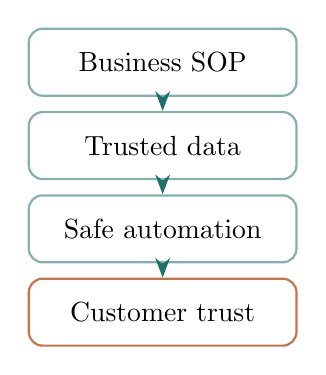
\begin{tikzpicture}[scale=0.92]
        \node[cardwhite,minimum width=3.4cm,minimum height=0.85cm] (sop) at (0,1.7) {Business SOP};
        \node[cardwhite,minimum width=3.4cm,minimum height=0.85cm] (data) at (0,0.55) {Trusted data};
        \node[cardwhite,minimum width=3.4cm,minimum height=0.85cm] (auto) at (0,-0.6) {Safe automation};
        \node[cardwhite,minimum width=3.4cm,minimum height=0.85cm,draw=terra] (trust) at (0,-1.75) {Customer trust};
        \draw[arrow] (sop) -- (data);
        \draw[arrow] (data) -- (auto);
        \draw[arrow] (auto) -- (trust);
      \end{tikzpicture}
      \end{center}
  \end{columns}
\end{frame}

% ---- 13. Future automations -----------------------------------------
\begin{frame}{What else we can automate later}
  \vspace{0.05cm}
  \begin{center}
  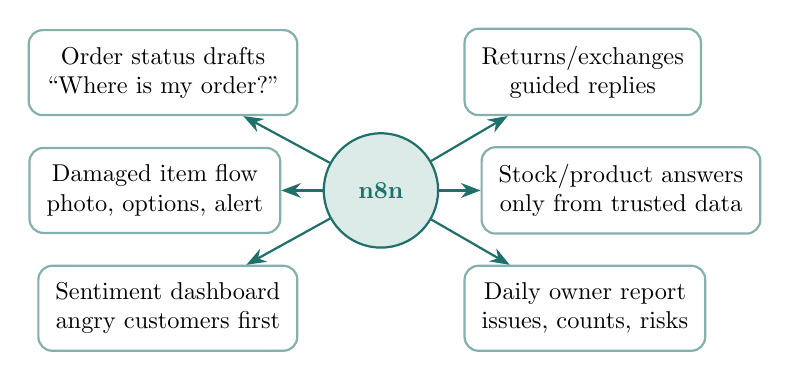
\begin{tikzpicture}[node distance=0.48cm and 0.6cm,scale=0.88,transform shape]
    \node[circle,draw=teal,thick,fill=softgreen,minimum size=1.65cm,font=\bfseries,text=teal] (core) {n8n};
    \node[cardwhite,above left=of core,minimum width=3.1cm] (wismo) {Order status drafts\\``Where is my order?''};
    \node[cardwhite,above right=of core,minimum width=3.1cm] (returns) {Returns/exchanges\\guided replies};
    \node[cardwhite,left=of core,minimum width=3.1cm] (damage) {Damaged item flow\\photo, options, alert};
    \node[cardwhite,right=of core,minimum width=3.1cm] (stock) {Stock/product answers\\only from trusted data};
    \node[cardwhite,below left=of core,minimum width=3.1cm] (sent) {Sentiment dashboard\\angry customers first};
    \node[cardwhite,below right=of core,minimum width=3.1cm] (report) {Daily owner report\\issues, counts, risks};
    \draw[arrow] (core) -- (wismo); \draw[arrow] (core) -- (returns);
    \draw[arrow] (core) -- (damage); \draw[arrow] (core) -- (stock);
    \draw[arrow] (core) -- (sent); \draw[arrow] (core) -- (report);
  \end{tikzpicture}
  \end{center}
\end{frame}

% ---- 14. Real-world example -----------------------------------------
\begin{frame}{Real-world example: order-status email}
  \vspace{0.1cm}
  \begin{block}{Customer says: ``Where is my order?''}
    A normal inbox makes someone manually check Gmail, Shopify and AusPost. Automation can do the checking first.
  \end{block}
  \vspace{0.35cm}
  \begin{center}
  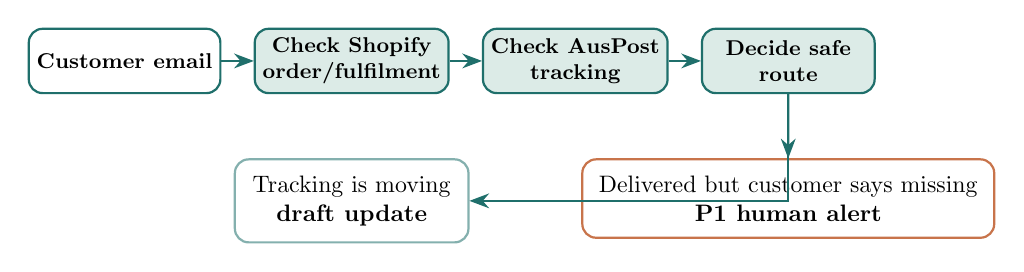
\begin{tikzpicture}[node distance=0.48cm,scale=0.86,transform shape]
    \node[route,fill=white] (cust) {Customer email};
    \node[route,right=of cust] (shop) {Check Shopify\\order/fulfilment};
    \node[route,right=of shop] (aus) {Check AusPost\\tracking};
    \node[route,right=of aus] (decide) {Decide safe\\route};
    \draw[arrow] (cust) -- (shop);
    \draw[arrow] (shop) -- (aus);
    \draw[arrow] (aus) -- (decide);

    \node[cardwhite,below=0.95cm of shop,minimum width=3.45cm] (safe) {Tracking is moving\\\textbf{draft update}};
    \node[cardwhite,below=0.95cm of decide,minimum width=3.65cm,draw=terra] (risk) {Delivered but customer says missing\\\textbf{P1 human alert}};
    \draw[arrow] (decide) |- (safe);
    \draw[arrow] (decide) -- (risk);
  \end{tikzpicture}
  \end{center}
  \vspace{0.2cm}
  \begin{center}
    \small\textcolor{muted}{This saves time but still protects the business when the situation is risky.}\\[0.25em]
    \tiny\textcolor{muted}{And it is mainstream in 2026: Shopify ships built-in automation (Flow), and shops adopting AI support report gains in cost, reply speed and satisfaction within 60--90 days. Sources: shopify.com/flow; Retail Technology Innovation Hub (2026); pctechmag.com (2026).}
  \end{center}
\end{frame}

% ---- 15. 90-day plan -------------------------------------------------
\begin{frame}{A practical 90-day plan}
  \vspace{0.1cm}
  \begin{center}
  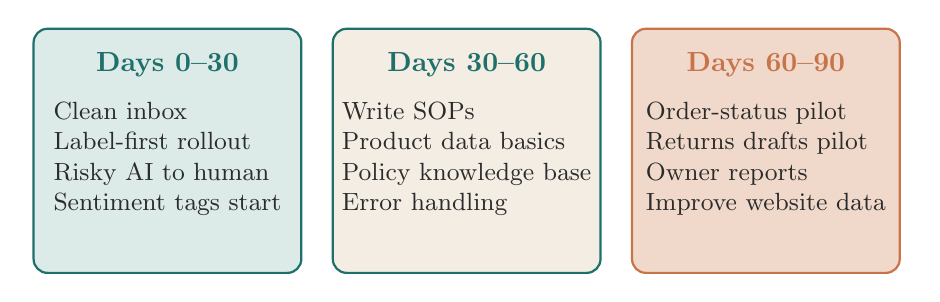
\begin{tikzpicture}[x=1cm,y=1cm]
    \draw[fill=softgreen,draw=teal,thick,rounded corners=5pt] (0,0) rectangle (3.4,3.1);
    \draw[fill=sand,draw=teal,thick,rounded corners=5pt] (3.8,0) rectangle (7.2,3.1);
    \draw[fill=softterra,draw=terra,thick,rounded corners=5pt] (7.6,0) rectangle (11,3.1);
    \node[font=\bfseries,text=teal] at (1.7,2.65) {Days 0--30};
    \node[font=\bfseries,text=teal] at (5.5,2.65) {Days 30--60};
    \node[font=\bfseries,text=terra] at (9.3,2.65) {Days 60--90};
    \node[align=left,font=\small,text=ink] at (1.7,1.45) {\begin{tabular}{l}Clean inbox\\Label-first rollout\\Risky AI to human\\Sentiment tags start\end{tabular}};
    \node[align=left,font=\small,text=ink] at (5.5,1.45) {\begin{tabular}{l}Write SOPs\\Product data basics\\Policy knowledge base\\Error handling\end{tabular}};
    \node[align=left,font=\small,text=ink] at (9.3,1.45) {\begin{tabular}{l}Order-status pilot\\Returns drafts pilot\\Owner reports\\Improve website data\end{tabular}};
  \end{tikzpicture}
  \end{center}
  \vspace{0.35cm}
  \begin{block}{Simple order of work}
    Relief first. Safety second. Bigger automation third.
  \end{block}
\end{frame}

% ---- 16. Business benefits ------------------------------------------
\begin{frame}{What the business gets}
  \vspace{0.05cm}
  \begin{center}
  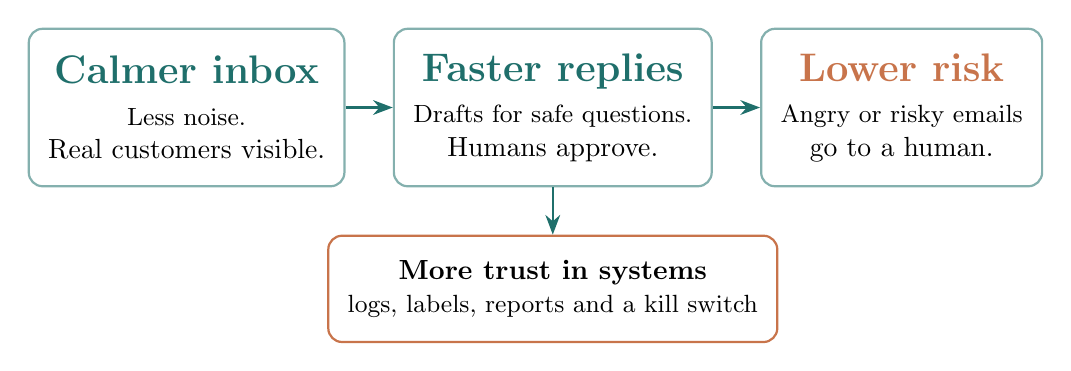
\begin{tikzpicture}[node distance=0.6cm]
    \node[cardwhite,minimum width=3.2cm,minimum height=2cm] (calm) {\Large\bfseries\textcolor{teal}{Calmer inbox}\\[0.3em]\small Less noise.\\Real customers visible.};
    \node[cardwhite,right=of calm,minimum width=3.2cm,minimum height=2cm] (fast) {\Large\bfseries\textcolor{teal}{Faster replies}\\[0.3em]\small Drafts for safe questions.\\Humans approve.};
    \node[cardwhite,right=of fast,minimum width=3.2cm,minimum height=2cm] (risk) {\Large\bfseries\textcolor{terra}{Lower risk}\\[0.3em]\small Angry or risky emails\\go to a human.};
    \node[cardwhite,below=of fast,minimum width=3.8cm,minimum height=1.35cm,draw=terra] (trust) {\bfseries More trust in systems\\\small logs, labels, reports and a kill switch};
    \draw[arrow] (calm) -- (fast);
    \draw[arrow] (fast) -- (risk);
    \draw[arrow] (fast) -- (trust);
  \end{tikzpicture}
  \end{center}
\end{frame}

% ---- 16b. Build vs Buy vs DIY ---------------------------------------
\begin{frame}{The honest question: build, buy, or do it yourself?}
  \vspace{0.1cm}
  \begin{center}
  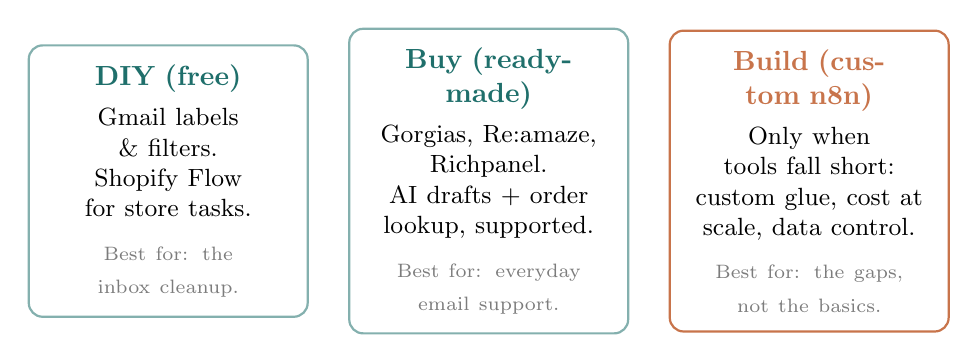
\begin{tikzpicture}[node distance=0.5cm]
    \node[cardwhite,minimum width=3.5cm,minimum height=2.9cm,text width=3.05cm] (diy)
      {\textbf{\textcolor{teal}{DIY (free)}}\\[0.35em]\small Gmail labels \& filters.\\Shopify Flow for store tasks.\\[0.4em]\scriptsize\textcolor{muted}{Best for: the inbox cleanup.}};
    \node[cardwhite,right=of diy,minimum width=3.5cm,minimum height=2.9cm,text width=3.05cm] (buy)
      {\textbf{\textcolor{teal}{Buy (ready-made)}}\\[0.35em]\small Gorgias, Re:amaze, Richpanel.\\AI drafts + order lookup, supported.\\[0.4em]\scriptsize\textcolor{muted}{Best for: everyday email support.}};
    \node[cardwhite,right=of buy,minimum width=3.5cm,minimum height=2.9cm,text width=3.05cm,draw=terra] (build)
      {\textbf{\textcolor{terra}{Build (custom n8n)}}\\[0.35em]\small Only when tools fall short:\\custom glue, cost at scale, data control.\\[0.4em]\scriptsize\textcolor{muted}{Best for: the gaps, not the basics.}};
  \end{tikzpicture}
  \end{center}
  \vspace{0.4cm}
  \begin{block}{The honest take}
    For most of this, the smart move is to buy or DIY --- not commission a custom black box. The value isn't building from scratch; it's choosing right and making it actually work for your shop.
  \end{block}
\end{frame}

% ---- 16c. Where I add value -----------------------------------------
\begin{frame}{Where I actually add value}
  \vspace{0.1cm}
  \begin{center}
  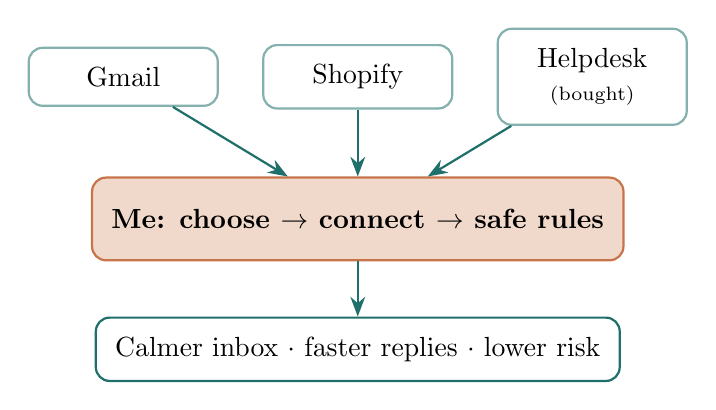
\begin{tikzpicture}[node distance=0.5cm and 0.55cm]
    \node[cardwhite,minimum width=2.4cm] (g) {Gmail};
    \node[cardwhite,right=of g,minimum width=2.4cm] (s) {Shopify};
    \node[cardwhite,right=of s,minimum width=2.4cm] (h) {Helpdesk\\\scriptsize(bought)};
    \node[card,below=0.85cm of s,minimum width=5.6cm,minimum height=1.05cm,draw=terra,fill=softterra] (me) {\bfseries Me: choose $\rightarrow$ connect $\rightarrow$ safe rules};
    \node[cardwhite,below=0.7cm of me,minimum width=5.6cm,draw=teal] (out) {Calmer inbox $\cdot$ faster replies $\cdot$ lower risk};
    \draw[arrow] (g) -- (me); \draw[arrow] (s) -- (me); \draw[arrow] (h) -- (me);
    \draw[arrow] (me) -- (out);
  \end{tikzpicture}
  \end{center}
  \vspace{0.25cm}
  \begin{itemize}\setlength\itemsep{0.38em}
    \item \textbf{Pick \& configure} the right tool --- not sell you a black box.
    \item \textbf{Write the SOPs} that make any tool safe (sizing, refunds, swaps).
    \item \textbf{Build only the glue} the tools can't do --- nothing reinvented.
    \item \textbf{No lock-in:} you own the tools, the data, and the rules.
  \end{itemize}
\end{frame}

% ---- 17. Engagement --------------------------------------------------
\begin{frame}{How I can keep helping}
  \vspace{0.2cm}
  \begin{columns}[T,onlytextwidth]
    \column{0.48\textwidth}
      \begin{block}{I can own the system work}
        \begin{itemize}\setlength\itemsep{0.35em}
          \item Gmail filters and labels.
          \item n8n workflow setup and hardening.
          \item AI prompt rules and safety checks.
          \item Google Sheets logs and reports.
          \item Shopify/AusPost/website data connections.
        \end{itemize}
      \end{block}
    \column{0.48\textwidth}
      \begin{block}{The business owns the rules}
        \begin{itemize}\setlength\itemsep{0.35em}
          \item Approve SOPs.
          \item Confirm policies.
          \item Confirm product facts.
          \item Decide what needs human approval.
          \item Review the first drafts before expanding.
        \end{itemize}
      \end{block}
  \end{columns}
  \vspace{0.3cm}
  \begin{center}\small\textcolor{muted}{That split keeps automation useful, safe and easy to trust.}\end{center}
\end{frame}

% ---- 18. Final ask ---------------------------------------------------
\begin{frame}{The ask: a small, paid discovery + setup sprint}
  \vspace{0.2cm}
  \begin{block}{Two weeks, fixed scope, clear deliverables}
    Start with the free inbox cleanup. Then I assess build-vs-buy for your support, set up the recommended tool, and write your first SOPs with you. You decide what comes next --- no open-ended commitment.
  \end{block}
  \vspace{0.45cm}
  \begin{center}
  
\begin{tikzpicture}[node distance=0.55cm]
    \node[cardwhite,minimum width=3.1cm,minimum height=1.45cm] (a) {\bfseries Free quick win\\\small Gmail cleanup};
    \node[cardwhite,right=of a,minimum width=3.1cm,minimum height=1.45cm] (b) {\bfseries Honest tool advice\\\small build vs buy};
    \node[cardwhite,right=of b,minimum width=3.1cm,minimum height=1.45cm,draw=terra] (c) {\bfseries First SOPs\\\small written with you};
    \draw[arrow] (a) -- (b);
    \draw[arrow] (b) -- (c);
  \end{tikzpicture}
  \end{center}
\end{frame}

% ---- Closing ---------------------------------------------------------
{
\setbeamercolor{background canvas}{bg=teal}
\begin{frame}[plain]
  \vspace{2.1cm}
  \begin{center}
    {\Huge\bfseries\textcolor{white}{Clean the noise.}}\\[0.45em]
    {\Huge\bfseries\textcolor{sand}{Build the engine.}}\\[0.75em]
    {\large\textcolor{sand}{Then automate only what the business can safely trust.}}\\[1.8em]
    \textcolor{terra}{\rule{5em}{2.5pt}}
  \end{center}
\end{frame}
}

\end{document}
